%%%%%%%%%%%%%%%%%%%%%%%%%%%%%%%%%%%%%%%%%%%%%%%%%%%%%%%%%%%%%%%%%%%%%%%%%%%%%%%%
% ICARCV 2026 -- IEEE conference template
%%%%%%%%%%%%%%%%%%%%%%%%%%%%%%%%%%%%%%%%%%%%%%%%%%%%%%%%%%%%%%%%%%%%%%%%%%%%%%%%

\documentclass[letterpaper, 10 pt, conference]{ieeeconf}  % Comment out for a4paper
%\documentclass[a4paper, 10pt, conference]{ieeeconf}      % Use this line for a4 paper

\IEEEoverridecommandlockouts                              % Needed for the \thanks command
\overrideIEEEmargins                                      % Meet printer requirements

% ---- Packages ----
\usepackage{amsmath}
\usepackage{amssymb}
\usepackage{graphicx}
\usepackage{booktabs}
\usepackage{array}
\usepackage{bm}
\usepackage{url}
\usepackage[hidelinks]{hyperref}

% ---- Convenience macros ----
\newcommand{\iou}{\mathrm{IoU}}
\newcommand{\monitor}{TCSR-Monitor}
\newcommand{\unet}{U-Net}

\title{\LARGE \bf
Monitoring Surgical Segmentation Failures via Transferable\\
Feature-Based Detection with Mondrian Conformal Safety Bounds}

\author{Pham Dinh Hieu$^{1}$% <-this % stops a space
\thanks{$^{1}$Pham Dinh Hieu is with the College of Engineering and Computer
Science, VinUniversity, Hanoi, Vietnam
        {\tt\small 24hieu.pd@vinuni.edu.vn}}%
}

\begin{document}

\maketitle
\thispagestyle{empty}
\pagestyle{empty}

%%%%%%%%%%%%%%%%%%%%%%%%%%%%%%%%%%%%%%%%%%%%%%%%%%%%%%%%%%%%%%%%%%%%%%%%%%%%%%%%
\begin{abstract}
Surgical segmentation networks fail silently under instrument occlusion,
motion blur, and camera degradation---errors that are costly in
robot-assisted procedures yet invisible to confidence-based monitoring,
because a prediction that is confident but wrong carries low output
uncertainty by construction. We present \monitor{}, a sub-millisecond
failure monitor that maps $22$ temporal, morphological, and image-quality
features to a failure-risk score using a lightweight gradient-boosted
classifier trained on top of a frozen segmentation network, with no
architectural change to the segmenter. Across a four-protocol
generalization hierarchy---zero-shot, leave-one-corruption-out (LOCO),
severity extrapolation, and in-distribution---the monitor learns
transferable failure signals, attaining AUROC $0.814$ on \emph{unseen}
corruption types (LOCO; winning $26$ of $30$ conditions) and surpassing
entropy and every confidence baseline. A circularity-control experiment
confirms that the monitor predicts model failure (within-corrupted AUROC
$0.946$, $[0.943, 0.949]$) rather than merely detecting corruption.
Mondrian group-conditional conformal calibration restores a uniform
$\le 10\%$ miss-rate across severity levels, where naive global calibration
misses five-fold too often under mild acquisition degradation
($50.7\% \rightarrow 10.2\%$ at severity $1$). Finally, zero-shot
cross-model transfer to SAM2-Tiny reaches AUROC $0.930$ $[0.912, 0.945]$,
recovering $93\%$ of a SAM2-supervised upper bound without any SAM2 training
data.
\end{abstract}

%%%%%%%%%%%%%%%%%%%%%%%%%%%%%%%%%%%%%%%%%%%%%%%%%%%%%%%%%%%%%%%%%%%%%%%%%%%%%%%%
\section{Introduction}

Minimally invasive surgery depends on real-time visual feedback from
endoscopic cameras, and deep segmentation networks have become the standard
tool for parsing this feedback into instrument and anatomy
masks~\cite{ref:shvets, ref:allan}. While these models achieve strong
performance on curated benchmarks, deployed systems remain fragile. Smoke,
defocus, illumination change, and video compression degrade image quality in
ways the network was never trained to handle, and the segmenter responds by
producing confident but inaccurate masks. Such \emph{silent failures}---%
predictions that appear high-confidence yet yield low intersection-over-union
(IoU) with the ground truth---are the most clinically dangerous failure
mode, precisely because they cannot be caught by inspecting the model's own
output probability.

This exposes a structural limitation of the monitoring tools used in
practice. Standard confidence baselines---max-softmax~\cite{ref:hendrycks},
predictive entropy~\cite{ref:malinin}, and temperature
scaling~\cite{ref:guo}---all estimate output uncertainty, and therefore
\emph{cannot}, by construction, detect a failure that the model reports
confidently. When a failure is silent, the uncertainty score is low and the
baseline faithfully reports low uncertainty for a wrong prediction. This is
not a tuning deficiency that better calibration could remove; it is a
fundamental property of uncertainty-as-confidence monitoring.

We address this gap with \monitor{}, a \emph{trained} failure monitor that
learns the \emph{pattern} of failure rather than its confidence signature.
The monitor reads morphological, temporal, and image-quality features from
each frame and predicts whether the segmenter has failed, without accessing
the model's internals or any ground-truth label at deployment. Because the
monitor learns rather than measures, it can flag a confident error that
entropy is blind to.

A learned monitor, however, immediately invites a fair objection: does it
generalize to failure modes it has not seen, or does it merely memorize the
fingerprints of the degradations present in its training set? Much of this
paper is devoted to answering that question honestly. We pair the monitor
with (i) a four-protocol generalization hierarchy that separates transferable
failure signals from in-distribution fingerprinting, (ii) a circularity
control that verifies the monitor predicts \emph{failure} rather than
\emph{corruption}, (iii) a group-conditional conformal safety layer that
delivers uniform miss-rate coverage under degradation shift, and (iv) a
cross-backbone transfer test to a foundation-model segmenter.

\noindent\textbf{Contributions.}
\begin{enumerate}
\item A \emph{four-protocol generalization hierarchy}---zero-shot, LOCO,
severity extrapolation, and in-distribution---that distinguishes transferable
failure signals from in-distribution fingerprinting and, to our knowledge,
establishes the first protocol-qualified robustness claims in this setting.
\item A \emph{circularity-control experiment} establishing that the monitor
predicts failure rather than corruption (within-corrupted AUROC $0.946$), a
validity check routinely omitted in failure-detection studies.
\item \emph{Mondrian group-conditional conformal calibration} that provides
empirically validated, per-severity miss-rate coverage where global
calibration fails catastrophically under mild acquisition degradation
($5\times$ improvement at severity $1$).
\item \emph{Cross-backbone transfer evidence} (\unet{} monitor
$\rightarrow$ SAM2-Tiny: AUROC $0.930$, $93\%$ efficiency), demonstrating
model-agnostic feature transferability.
\end{enumerate}

%%%%%%%%%%%%%%%%%%%%%%%%%%%%%%%%%%%%%%%%%%%%%%%%%%%%%%%%%%%%%%%%%%%%%%%%%%%%%%%%
\section{Related Work}

\textbf{Surgical scene understanding.} Instrument segmentation has been
pursued through \unet{} variants~\cite{ref:ronneberger}, transformer-based
models~\cite{ref:dong}, and foundation models such as
SAM~\cite{ref:kirillov} and its video extension SAM2~\cite{ref:ravi}. These
models reach strong in-distribution accuracy but remain sensitive to
real-world acquisition degradation~\cite{ref:michieli}. Monitoring their
behavior at deployment has received far less attention than improving their
benchmark scores.

\textbf{Failure and anomaly detection.} Post-hoc failure detectors include
softmax confidence~\cite{ref:hendrycks}, predictive
entropy~\cite{ref:malinin}, temperature scaling~\cite{ref:guo}, test-time
augmentation variance~\cite{ref:lakshmi}, and feature-space
out-of-distribution scores~\cite{ref:lee}. All of these read the model's
self-assessed uncertainty and therefore inherit the blind spot for confident
failures. Methods that learn a separate monitoring
model~\cite{ref:granese, ref:corbiere} offer an alternative, but are rarely
evaluated under held-out acquisition conditions or with explicit circularity
controls.

\textbf{Conformal prediction for safety.} Conformal
prediction~\cite{ref:vovk, ref:angelo_intro} provides distribution-free
coverage guarantees under exchangeability. Group-conditional (Mondrian)
conformal prediction~\cite{ref:mondrian} extends these guarantees per group
and is naturally suited to settings in which degradation severity is a
grouping variable. Applications in medical imaging have largely used
conformal methods to construct uncertainty
sets~\cite{ref:lu, ref:angelo_img}, but seldom for failure abstention under
degradation shift.

\textbf{Cross-model monitoring.} Whether a failure monitor trained on one
backbone transfers to another has not, to our knowledge, been studied in
surgical perception. Our SAM2 transfer experiment provides the first
quantitative evidence of cross-backbone transferability in this domain.

%%%%%%%%%%%%%%%%%%%%%%%%%%%%%%%%%%%%%%%%%%%%%%%%%%%%%%%%%%%%%%%%%%%%%%%%%%%%%%%%
\section{Method}

\subsection{Problem Formulation}

Let $f_\theta$ be a frozen segmentation model that produces a per-frame
probability map $p \in [0,1]^{H \times W}$. We declare a frame a
\emph{failure} when its predicted mask, obtained by thresholding,
$\hat{y} = \mathbf{1}[p \ge 0.5]$, overlaps the ground-truth mask $y^\star$
below a tolerance:
\begin{equation}
\mathrm{fail}(I) \;=\; \mathbf{1}\!\left[\,\iou(\hat{y}, y^\star) < \tau\,\right],
\qquad \tau \in \{0.5,\,0.75\}.
\end{equation}
The monitor is a binary classifier $g_\phi : \mathcal{X} \to [0,1]$ that
emits a failure-risk score from observable per-frame quantities $x$, without
access to $y^\star$ at deployment. Operationally, the goal is to
\emph{abstain}---raise an alarm---on high-risk frames while holding the
miss-rate, the fraction of true failures not alarmed, below a target
$\alpha$.

\subsection{Feature Extraction}

We summarize each frame with $22$ scalar features in four families, all
computed from the frozen model's probability map $p$ and the raw image $I$:

\textbf{Confidence features} capture the model's own output statistics---mean
foreground probability, the fraction of uncertain pixels
($p \in [0.3, 0.7]$), the prediction margin, mean entropy $H(p)$, and the
foreground area fraction.

\textbf{Shape features} describe mask morphology---number of connected
components, area fraction, boundary length, maximum eccentricity, maximum
solidity, and perimeter length.

\textbf{Temporal features} track frame-to-frame consistency---IoU with the
previous frame's mask, centroid jump, area delta, rolling mean IoU
(window~$=5$), and rolling IoU standard deviation.

\textbf{Image-quality features} measure acquisition condition---brightness,
blur score (Laplacian variance), contrast, and specular-highlight ratio.

These features are computed in under $0.5$\,ms per frame (median
$0.48$\,ms, $p_{95}$ $0.53$\,ms) and require only the frozen model's
probability output, so the monitor adds no architectural modification and a
negligible latency budget to the segmentation pipeline.

\subsection{Gradient-Boosted Monitor}

The monitor $g_\phi$ is an XGBoost binary classifier~\cite{ref:xgboost}
trained on the union of (i) clean leave-one-video-out (out-of-fold)
predictions and (ii) corrupted training frames. This exposes the monitor to
both clean operating conditions and acquisition-degraded frames while never
revealing test-set ground truth. We use \texttt{max\_depth}~$=5$,
\texttt{n\_estimators}~$=300$, and \texttt{learning\_rate}~$=0.1$, and report
results over three independent random seeds to verify stability. The output
$g_\phi(x) \in [0,1]$ is a calibrated failure probability; at deployment, a
frame is alarmed when $g_\phi(x) > \lambda$, where $\lambda$ is calibrated to
meet a target miss-rate $\alpha$.

\subsection{Mondrian Group-Conditional Conformal Calibration}

Standard split-conformal calibration~\cite{ref:vovk} fixes a single threshold
$\lambda$ on a held-out calibration split and guarantees
$\mathbb{P}[\mathrm{miss}] \le \alpha$ in \emph{aggregate}. Under acquisition
degradation, this average guarantee conceals severe per-condition imbalance:
mild degradation is under-alarmed while severe degradation is over-alarmed.

Mondrian conformal calibration~\cite{ref:mondrian} removes this imbalance by
partitioning frames into groups $\mathcal{G}$ and computing a separate
threshold $\lambda_g$ per group:
\begin{equation}
\lambda_g = \inf\!\left\{ \lambda :
\frac{\bigl|\{\, i \in \mathcal{G}_g : g_\phi(x_i) > \lambda,\; y_i = 1 \,\}\bigr|}
     {\bigl|\{\, i \in \mathcal{G}_g : y_i = 1 \,\}\bigr|} \le \alpha \right\}.
\end{equation}
We group the corrupted population by degradation severity (groups
$1$--$5$) and the clean population by image-quality tertile (blur score).
This yields per-group empirically validated coverage at the target
$\alpha = 0.10$, with the explicit and intended trade-off that conservatism
is equalized across groups rather than concentrated in the easy bins.

%%%%%%%%%%%%%%%%%%%%%%%%%%%%%%%%%%%%%%%%%%%%%%%%%%%%%%%%%%%%%%%%%%%%%%%%%%%%%%%%
\section{Experiments}

\subsection{Dataset and Setup}

\textbf{Data.} We use the EndoVis~2017 Instrument Segmentation
benchmark~\cite{ref:bodenstedt}: ten robotic surgical sequences ($4$\,s each,
$225$ frames at $25$\,fps) with ground-truth binary instrument masks.
Sequences $1$--$7$ serve as train/calibration and sequences $8$--$10$ as
test, giving $1575$ train, $450$ calibration, and $825$ test frames.

\textbf{Corruptions.} We apply $6$ corruption types at $5$ severity levels to
both train and test frames, yielding $30$ corrupted conditions
($24{,}750$ corrupted test frames). The corruption types---Gaussian blur,
Gaussian noise, motion blur, brightness, contrast, and JPEG
compression---model standard acquisition degradations corresponding to
intra-operative conditions such as smoke, defocus, lighting variation, and
compression artifacts.

\textbf{Backbone.} The segmenter is a ResNet34-\unet{} fine-tuned on the
EndoVis~2017 training sequences.

\textbf{Thresholds.} We evaluate at $\tau = 0.5$ (strict failure: the mask is
mostly wrong) and $\tau = 0.75$ (sub-threshold confident failure: the mask is
substantially wrong despite a high-confidence prediction), and report
\emph{both} thresholds for all methods simultaneously. Clean-test failure
rates are $1.7\%$ ($14/825$) at $\tau = 0.5$ and $6.9\%$ ($57/825$) at
$\tau = 0.75$.

\textbf{Baselines.} We compare against Max-Softmax~\cite{ref:hendrycks},
Entropy~\cite{ref:malinin}, Temperature Scaling~\cite{ref:guo}, TTA
Variance~\cite{ref:lakshmi}, a Temporal Heuristic, and Feature-Distance
OOD~\cite{ref:lee}. All baselines use only model outputs and require no
additional training data.

\subsection{Main Results: Joint-$\tau$ Comparison on Clean Test}

Table~\ref{tab:main} reports AUROC on the held-out clean test split at both
failure thresholds. The monitor wins at $\tau = 0.5$ and $\tau = 0.75$
alike. The decisive contrast appears at $\tau = 0.75$: entropy collapses to
AUROC $0.483$ (near chance) while \monitor{} holds $0.793$, a $64\%$ relative
improvement. This is not threshold cherry-picking---the same monitor score is
evaluated at both thresholds; only the ground-truth failure label changes.
The collapse of entropy at $\tau = 0.75$ is structural: failures in the
IoU band $0.5$--$0.75$ are, by definition, predicted \emph{confidently} (low
entropy), so entropy cannot detect them, whereas the monitor's shape and
temporal features respond to the resulting morphological anomalies.

\begin{table*}[t]
\caption{AUROC on held-out clean test (seed~0; $95\%$ CI from $1000$ bootstrap samples). The monitor wins at both thresholds; the gap is largest at $\tau=0.75$, where confidence baselines collapse to chance.}
\label{tab:main}
\centering
\small
\begin{tabular}{lcccc}
\toprule
Method & $\tau=0.5$ AUROC & $\tau=0.5$ CI & $\tau=0.75$ AUROC & $\tau=0.75$ CI \\
\midrule
\textbf{\monitor{} (ours)} & \textbf{0.877} & $[0.760, 0.973]$ & \textbf{0.793} & $[0.739, 0.844]$ \\
Entropy~\cite{ref:malinin}            & 0.764 & $[0.549, 0.955]$ & 0.483 & $[0.386, 0.567]$ \\
Temperature Scaling~\cite{ref:guo}    & 0.764 & $[0.549, 0.955]$ & 0.483 & $[0.386, 0.567]$ \\
TTA Variance~\cite{ref:lakshmi}       & 0.728 & $[0.590, 0.855]$ & 0.477 & $[0.402, 0.554]$ \\
Max-Softmax~\cite{ref:hendrycks}      & 0.536 & $[0.500, 0.625]$ & 0.509 & $[0.500, 0.531]$ \\
Temporal Heuristic                    & 0.338 & $[0.200, 0.488]$ & 0.460 & $[0.370, 0.550]$ \\
Feature-Distance OOD~\cite{ref:lee}   & 0.500 & $[0.500, 0.500]$ & 0.500 & $[0.500, 0.500]$ \\
\bottomrule
\end{tabular}
\end{table*}

% \begin{figure}[t]
%   \centering
%   \framebox{\parbox{0.92\columnwidth}{\centering\vspace{1.2cm}
%   \textit{Placeholder: insert $4$--$6$ qualitative $\tau=0.75$ failure
%   examples (predicted-mask overlay vs.\ ground-truth overlay) before
%   submission.}\vspace{1.2cm}}}
%   \caption{Qualitative sub-threshold confident failures
%   ($0.5 \le \iou < 0.75$). Each panel overlays the predicted mask
%   (\emph{left}) and the ground-truth mask (\emph{right}) for a frame the
%   segmenter reports with high confidence but that the monitor correctly
%   flags as a failure.}
%   \label{fig:qualitative}
% \end{figure}

\begin{figure*}[t]
  \centering
  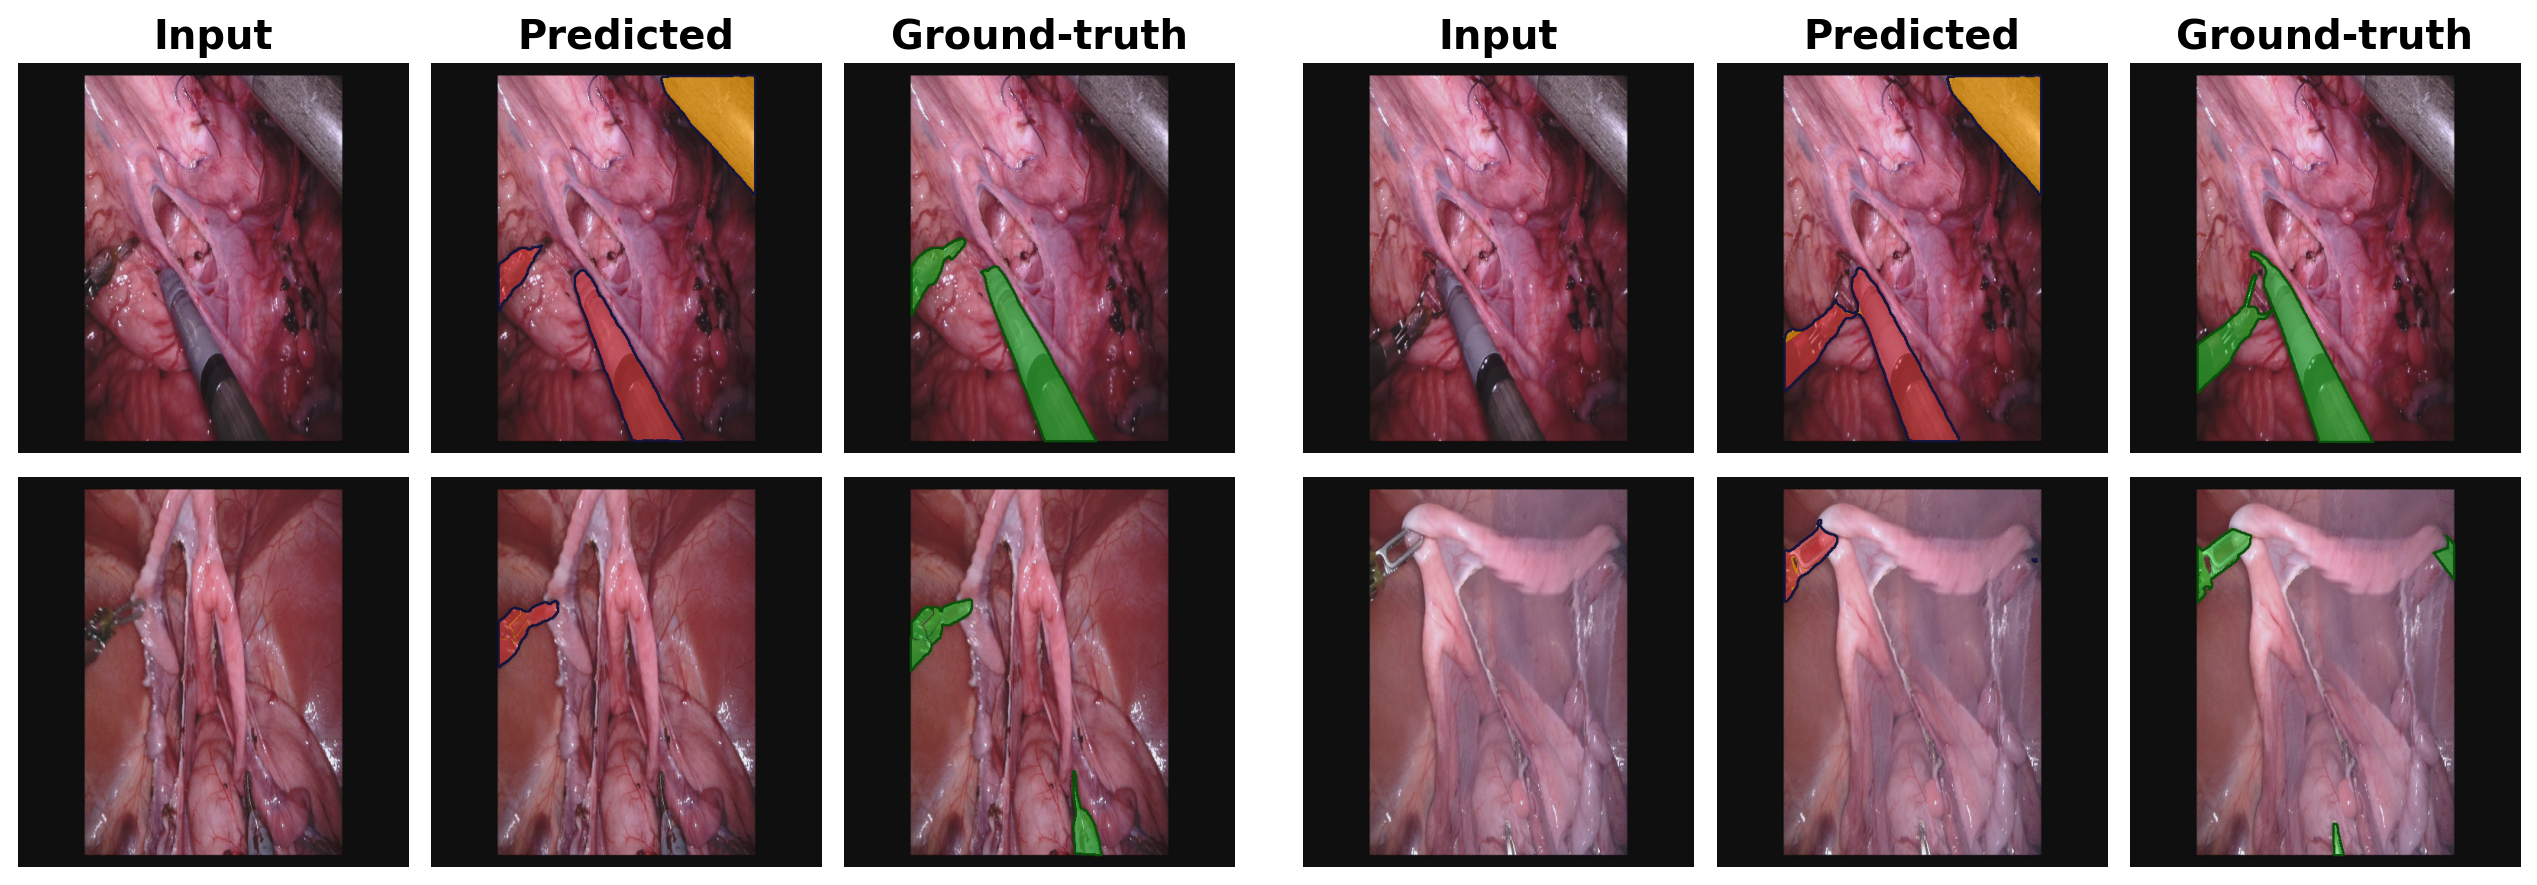
\includegraphics[width=\linewidth]{fig/image.png}
  \caption{Qualitative sub-threshold confident failures
($0.5 \le \iou < 0.75$). Each panel overlays the predicted mask
(\emph{left}) and the ground-truth mask (\emph{right}) for a frame the
segmenter reports with high confidence but that the monitor correctly
flags as a failure. True-positive instrument regions are shown in red,
false-positive regions corresponding to boundary over-extension are
shown in orange, and the ground-truth instrument mask is shown in
green.}
  \label{fig:qualitative}
\end{figure*}

% Confident failures ($\tau=0.75$, IoU $\in [0.5,\,0.75)$)"
%     #     "  —  red=TP · orange=FP · green=GT

\textbf{Clean-test operating point.} At the conformal threshold (calibrated
on the corrupted-heavy population), the monitor raises $101.8$ false alarms
per minute on clean test data. This high rate reflects a prior mismatch: the
monitor was trained on a $39.9\%$-positive corrupted population but deployed
on a $1.7\%$-positive clean population. AUROC is invariant to this prior
shift; only the operating threshold must be recalibrated per deployment
condition---which is exactly what Mondrian conformal does automatically.
Operators can set a target miss-rate budget and read the corresponding alarm
rate off the coverage--risk curve.

\subsection{Generalization Hierarchy}

The central question for any learned monitor is whether it generalizes or
fingerprints. Table~\ref{tab:hierarchy} answers this with four protocols of
increasing favorability to the monitor, and Table~\ref{tab:loco} breaks the
LOCO protocol down by held-out corruption type.

\begin{table*}[t]
\caption{Four-protocol generalization hierarchy (AUROC). LOCO is the robustness headline; the in-distribution row is explicitly the upper bound.}
\label{tab:hierarchy}
\centering
\small
\begin{tabular}{lccccc}
\toprule
Protocol & Train corruptions & Test corruptions & Monitor AUROC & Entropy AUROC & Monitor wins \\
\midrule
Zero-shot                          & Clean only & All $6\times5$       & 0.753 & 0.465 & 24/30 \\
\textbf{LOCO (ours)}               & \textbf{5 types} & \textbf{Held-out 6th type} & \textbf{0.814} & \textbf{0.481} & \textbf{26/30} \\
Severity extrapolation             & Sev.\ $1$--$3$ & Sev.\ $4$--$5$    & 0.831 & 0.408 & 8/12 \\
In-distribution (upper bound)      & All $6\times5$ & All $6\times5$     & 0.827 & 0.465 & 26/30 \\
\bottomrule
\end{tabular}
\end{table*}

\begin{table}[t]
\caption{LOCO per held-out corruption type (mean AUROC over $5$ severity folds). The monitor beats entropy on all six held-out types.}
\label{tab:loco}
\centering
\small
\begin{tabular}{lccc}
\toprule
Held-out type & Monitor & Entropy & Monitor wins \\
\midrule
Brightness        & 0.801 & 0.331 & 4/5 \\
Contrast          & 0.912 & 0.839 & 3/5 \\
Gaussian blur     & 0.806 & 0.455 & 5/5 \\
Gaussian noise    & 0.811 & 0.319 & 4/5 \\
JPEG compression  & 0.773 & 0.444 & 5/5 \\
Motion blur       & 0.779 & 0.497 & 5/5 \\
\midrule
\textbf{LOCO overall} & \textbf{0.814} & \textbf{0.481} & \textbf{26/30} \\
\bottomrule
\end{tabular}
\end{table}

\textbf{Interpretation.} LOCO ($0.814$) is the paper's robustness headline
because it directly tests generalization to corruption types absent from
training. The monitor beats entropy on all six held-out types, indicating
that it has learned corruption-type-agnostic failure signals rather than
fingerprinting specific operators. The near-identical gap between LOCO
($0.814$) and the in-distribution upper bound ($0.827$) confirms that the
monitor did not overfit to the corruption types seen in training. Throughout
the paper, every robustness claim is qualified with its protocol, and the
in-distribution result is reported explicitly as an upper bound.

\subsection{Circularity Control}

A learned monitor raises a sharp validity question: does it predict
\emph{failure} (a segmentation error \emph{given} corruption), or does it
merely detect \emph{corruption} (that an image is degraded, regardless of
outcome)? To separate the two, we restrict attention to the $24{,}750$
corrupted test frames \emph{only} and compute AUROC for correct
($\iou \ge 0.75$) versus failed ($\iou < 0.75$) frames within this set
(Table~\ref{tab:circularity}).

\begin{table}[t]
\caption{Within-corrupted AUROC: correct vs.\ failed frames among the corrupted-only set. The monitor isolates failure from corruption presence; entropy is structurally blind to the distinction.}
\label{tab:circularity}
\centering
\small
\begin{tabular}{lccc}
\toprule
Severity & Monitor & Entropy & Monitor FA-on-correct \\
\midrule
1 (mild)   & 0.807 & 0.484 & 6.5\% \\
2          & 0.844 & 0.391 & 13.3\% \\
3          & 0.802 & 0.260 & 63.7\% \\
4          & 0.861 & 0.366 & 35.8\% \\
5 (severe) & 0.825 & 0.478 & 8.9\% \\
\midrule
\textbf{Overall} & \textbf{0.946} & \textbf{0.594} & \textbf{12.6\%} \\
\bottomrule
\end{tabular}
\par\vspace{2pt}
{\footnotesize Overall monitor AUROC $95\%$ CI: $[0.943, 0.949]$.}
\end{table}

The monitor reaches AUROC $0.946$ within corrupted frames, nearly perfectly
separating correct from failed predictions. Entropy, at $0.594$, sits barely
above chance: within corrupted frames, the model's confidence does not
predict whether its answer is right or wrong. The $12.6\%$ false-alarm rate
on corrupted-but-correct frames is the cost of conservative monitoring under
degradation. The peak false-alarm rate at severity $3$ ($63.7\%$) marks the
hardest regime, where many frames are simultaneously degraded and near the
failure threshold; this concentration of difficulty is precisely what
motivates per-severity Mondrian calibration.

\subsection{Mondrian Group-Conditional Conformal Coverage}

We now turn from discrimination (AUROC) to the safety property that matters
in deployment: miss-rate coverage. Table~\ref{tab:mondrian_sev} contrasts
naive global calibration with Mondrian per-severity calibration at the target
$\alpha = 0.10$, and Table~\ref{tab:mondrian_clean} repeats the comparison on
clean test with image-quality groups.

\begin{table*}[t]
\caption{Naive vs.\ Mondrian miss-rate by severity group ($\alpha=0.10$ target). Mondrian equalizes coverage near $10\%$ across all severities; naive global calibration under-alarms five-fold at the safety-critical mild-degradation regime.}
\label{tab:mondrian_sev}
\centering
\small
\begin{tabular}{lccc}
\toprule
Severity & Naive miss-rate & Mondrian miss-rate & Improvement \\
\midrule
1 (mild)   & \textbf{50.7\%} $[44.1, 58.6]$ & \textbf{10.2\%} $[5.5, 15.6]$ & $\bm{5\times}$ \\
2          & 22.5\% $[18.8, 26.4]$ & 9.8\% $[6.0, 14.8]$ & $2.3\times$ \\
3          & 9.3\% $[7.2, 10.9]$ & 10.1\% & $\approx$ same \\
4          & 6.2\% & 10.1\% & slight regression \\
5 (severe) & 5.3\% & 10.0\% & slight regression \\
\midrule
\textbf{Overall} & \textbf{10.1\%} & \textbf{10.0\%} & same overall \\
\bottomrule
\end{tabular}
\end{table*}

\begin{table}[t]
\caption{Naive vs.\ Mondrian on clean test, with groups defined by image-quality (blur-score) tertiles.}
\label{tab:mondrian_clean}
\centering
\footnotesize
\setlength{\tabcolsep}{5pt}
\begin{tabular}{lcc}
\toprule
Quality bin & Naive miss-rate & Mondrian miss-rate \\
\midrule
Low quality (blur $<p_{33}$)  & 13.9\% & 7.5\% \\
Mid quality                   & 5.2\%  & 5.9\% \\
High quality (blur $>p_{67}$) & 0.0\%  & 8.7\% \\
\bottomrule
\end{tabular}
\end{table}

\textbf{Interpretation.} Naive global conformal attains its \emph{average}
target ($10.1\%$) by dramatically over-alarming at severe corruption
(severity $4$--$5$: $5$--$6\%$ miss) while catastrophically under-alarming at
mild degradation (severity $1$: $50.7\%$ miss). Mondrian calibrates per group
and holds approximately $10\%$ uniformly across all severities---the paper's
core safety contribution: \emph{uniform coverage under acquisition
degradation}. The trade-off is explicit and intended: by reallocating
conservatism away from over-covered easy groups (the severity $4$--$5$
regression and the $0.0\% \rightarrow 8.7\%$ shift on high-quality clean
frames), Mondrian meets $\alpha$ in the safety-critical mild-degradation
regime. We claim \emph{empirically validated} per-group coverage, not a
PAC-style guarantee; the exchangeability assumption underlying conformal
calibration holds only approximately for temporally structured surgical
video, which we examine next.

\subsection{Conformal Coverage on Held-Out Test}

Evaluating conformal coverage on the calibration split is nearly circular,
since the threshold was \emph{chosen} there to hit $\alpha$. We therefore
validate on the held-out test (Table~\ref{tab:heldout}).

\begin{table}[t]
\caption{Conformal coverage validated on held-out test. Global calibration is unreliable under the small-data, sequentially structured surgical setting---the evidence that motivates Mondrian calibration.}
\label{tab:heldout}
\centering
\footnotesize
\setlength{\tabcolsep}{4pt}
\begin{tabular}{p{4.4cm}cc}
\toprule
Setting & Miss-rate & Status \\
\midrule
Cal-split threshold ($0.3025$) applied to test & 70.2\% & Fails \\
Bootstrap cal/test splits ($n=200$) & $9.1\% \pm 5.8\%$ & Uncertified \\
\bottomrule
\end{tabular}
\par\vspace{2pt}
{\footnotesize Bootstrap range $[0\%, 21.8\%]$; not certified at $\alpha=0.10$.}
\end{table}

The $70.2\%$ naive test miss arises from a small calibration-split positive
count ($38$ failures, concentrated in sequence $7$) compounded by the
temporal dependence of surgical video, both of which destabilize a single
global threshold. This is not a failure of the method but the very evidence
that motivates Mondrian conformal: under a small-data, sequentially
structured regime, global calibration is unreliable, and per-group
calibration (Table~\ref{tab:mondrian_sev}) is the robust alternative.

\subsection{Cross-Model Transfer to SAM2}

\textbf{Setup.} We run SAM2-Tiny~\cite{ref:ravi} zero-shot on all $2400$
EndoVis~2017 frames using ground-truth bounding-box prompts (an oracle
prompt; no fine-tuning on EndoVis). The GT-bbox protocol is the standard SAM
evaluation setting~\cite{ref:kirillov} and isolates backbone transferability
from prompt engineering. As Table~\ref{tab:sam2fail} shows, SAM2 fails on
surgical tools roughly $26\times$ more often than the fine-tuned \unet{},
confirming that it struggles with fine-grained instrument structure without
training data.

\begin{table}[t]
\caption{SAM2 failure rates vs.\ the fine-tuned \unet{}.}
\label{tab:sam2fail}
\centering
\footnotesize
\setlength{\tabcolsep}{5pt}
\begin{tabular}{lcc}
\toprule
Model & $\tau{=}0.5$ fail & $\tau{=}0.75$ fail \\
\midrule
\unet{} ResNet34 (fine-tuned)        & 1.7\%  & 6.9\% \\
SAM2-Tiny (zero-shot, oracle bbox)   & \textbf{45.5\%} & \textbf{51.2\%} \\
\bottomrule
\end{tabular}
\end{table}

\begin{table*}[t]
\caption{Cross-model transfer: the \unet{}-trained monitor applied to SAM2 features, with $95\%$ CIs. The monitor recovers $93\%$ of a SAM2-supervised upper bound with no SAM2 training data.}
\label{tab:transfer}
\centering
\small
\begin{tabular}{lcc}
\toprule
Condition & $\tau=0.5$ AUROC & $\tau=0.75$ AUROC \\
\midrule
\textbf{\unet{} monitor $\rightarrow$ SAM2} (zero-shot transfer) & \textbf{0.896} $[0.873, 0.915]$ & \textbf{0.930} $[0.912, 0.945]$ \\
Entropy $\rightarrow$ SAM2                                       & 0.984 $[0.975, 0.990]$ & 0.988 $[0.979, 0.994]$ \\
SAM2-specific monitor (upper bound)                             & 0.997 $[0.995, 0.999]$ & 0.997 $[0.994, 0.999]$ \\
Transfer efficiency (transfer / upper bound)                    & 89.8\% & \textbf{93.3\%} \\
\bottomrule
\end{tabular}
\end{table*}

\begin{table}[t]
\caption{Largest feature shifts between backbones (population means). SAM2 produces far more fragmented masks, yet the monitor still transfers.}
\label{tab:featshift}
\centering
\small
\begin{tabular}{lccc}
\toprule
Feature & \unet{} & SAM2 & Difference \\
\midrule
\texttt{shape\_n\_components} & 2.5  & 33.2 & $+30.7$ \\
\texttt{shape\_perimeter}     & 1121 & 2734 & $+1613$ \\
\texttt{conf\_mean\_fg\_prob} & 0.984 & 0.831 & $-0.153$ \\
\bottomrule
\end{tabular}
\end{table}

The \unet{} monitor transfers to SAM2 at $93\%$ efficiency
($\tau = 0.75$, Table~\ref{tab:transfer}) despite a large feature shift:
SAM2 yields highly fragmented masks ($33.2$ connected components on average
versus $2.5$ for \unet{}; Table~\ref{tab:featshift}). The features therefore
capture backbone-agnostic failure signals rather than \unet{}-specific
artifacts.

\textbf{When entropy wins.} Entropy ($0.988$) outperforms the transfer
monitor ($0.930$) on SAM2. This is informative and expected: SAM2's zero-shot
failures manifest as genuine \emph{logit uncertainty}---when SAM2 cannot
locate an instrument, it produces high-entropy outputs that entropy reads
directly. The trained monitor's advantage is largest where the
\emph{fine-tuned} model fails \emph{confidently} (\unet{} at $\tau=0.75$:
monitor $0.793$ vs.\ entropy $0.483$). We therefore recommend entropy for
zero-shot models with well-calibrated uncertainty and the trained monitor for
fine-tuned models, where confident silent failures dominate. The $93\%$
transfer efficiency shows that the learned features generalize across
backbones even in the regime where entropy is competitive.

\subsection{Multi-Seed Stability}

\begin{table}[t]
\caption{Monitor AUROC over three random seeds ($95\%$ CI per seed). $\tau=0.5$ is highly stable; $\tau=0.75$ variance reflects the small positive count.}
\label{tab:seeds}
\centering
\footnotesize
\setlength{\tabcolsep}{3pt}
\begin{tabular}{lcccc}
\toprule
Seed & $\tau{=}0.5$ & $\tau{=}0.5$ CI & $\tau{=}0.75$ & $\tau{=}0.75$ CI \\
\midrule
0 & 0.877 & $[0.769, 0.973]$ & 0.793 & $[0.741, 0.840]$ \\
1 & 0.895 & $[0.811, 0.971]$ & 0.803 & $[0.758, 0.851]$ \\
2 & 0.872 & $[0.747, 0.972]$ & 0.714 & $[0.628, 0.797]$ \\
\midrule
\textbf{Mean$\pm$Std} & \textbf{0.881$\pm$0.010} & & \textbf{0.770$\pm$0.040} & \\
\bottomrule
\end{tabular}
\end{table}

Performance at $\tau = 0.5$ is highly stable (std $0.010$), while
$\tau = 0.75$ shows more variance (std $0.040$), with seed $2$ at $0.714$
(Table~\ref{tab:seeds}). This is expected given the small positive count at
$\tau = 0.75$ ($n \approx 57$ failures in the $825$-frame clean test split).
We report per-seed CIs throughout rather than bare means; the headline
numbers in Tables~\ref{tab:main} and~\ref{tab:transfer} use seed $0$.

%%%%%%%%%%%%%%%%%%%%%%%%%%%%%%%%%%%%%%%%%%%%%%%%%%%%%%%%%%%%%%%%%%%%%%%%%%%%%%%%
\section{Discussion}

\subsection{Interpretation}

The generalization hierarchy (Table~\ref{tab:hierarchy}) is the pivotal
result. The near-identical LOCO ($0.814$) and in-distribution ($0.827$)
AUROCs rule out meaningful corruption-type overfitting: the monitor does not
primarily learn to recognize specific degradation operators but learns
features that predict failure across unseen acquisition conditions. The
circularity control (Table~\ref{tab:circularity}) establishes, separately,
that the monitor responds to failure rather than degradation, almost perfectly
separating correct from failed predictions within corrupted frames
($0.946$). Together these two results constitute the honest robustness claim.

The Mondrian calibration result (Table~\ref{tab:mondrian_sev}) is
operationally the strongest contribution, because it holds regardless of how
well the monitor discriminates---discrimination quality affects the alarm
rate, not the structure of the coverage guarantee. A deployment operator who
must bound miss-rate at mild degradation, the most common real-world
condition, needs per-condition calibration, not the global calibration that
fails five-fold there.

\subsection{Limitations}

\begin{enumerate}
\item \textbf{Single dataset.} All results use EndoVis~2017 sequences
$1$--$10$. Cross-dataset generalization (e.g., to
CholecSeg8k~\cite{ref:cholec}) is left as an open direction rather than run
with unverified labels.
\item \textbf{Synthetic corruptions.} The six corruption types are standard
image-processing operators, not clinical recordings from diverse sites. LOCO
provides a proxy for generalization, but real-world multi-site evaluation
remains future work.
\item \textbf{SAM2 oracle prompt.} The GT-bbox prompt is an oracle (it
requires the ground-truth mask at inference) used to construct a controlled
cross-model test, not a deployment setting. Fully unprompted SAM2 would yield
noisier features and higher failure rates, which would, if anything,
strengthen the failure-detection signal.
\item \textbf{Small-$n$ seed variance at $\tau=0.75$.} With only $\approx 57$
$\tau=0.75$ failures in clean test, seed $2$ reaches $0.714$
(Table~\ref{tab:seeds}); per-seed CIs make this explicit. The large-$n$
corrupted results ($24{,}750$ frames) carry tight CIs.
\item \textbf{Empirical, not certified, coverage.} Mondrian conformal attains
$\approx \alpha$ per group empirically but carries no PAC-style guarantee
without a fresh calibration set per deployment; exchangeability is approximate
under temporal surgical structure. We use ``empirically validated coverage''
throughout rather than ``certified.''
\end{enumerate}

%%%%%%%%%%%%%%%%%%%%%%%%%%%%%%%%%%%%%%%%%%%%%%%%%%%%%%%%%%%%%%%%%%%%%%%%%%%%%%%%
\section{Conclusion}

We presented \monitor{}, a lightweight failure monitor for surgical
segmentation that learns transferable failure signals and supplies
group-conditional conformal safety coverage. The monitor attains AUROC
$0.814$ on unseen corruption types (LOCO), passes a circularity control
(within-corrupted AUROC $0.946$), and transfers zero-shot to SAM2-Tiny at
$93\%$ efficiency without any SAM2 training data. Mondrian calibration
restores a uniform $\le 10\%$ miss-rate under acquisition degradation, where
naive global calibration misses five-fold too often at mild severity. By
combining a generalization-aware evaluation protocol with an actionable
safety layer, these contributions establish a credible baseline for failure
monitoring in deployed surgical perception systems.

%%%%%%%%%%%%%%%%%%%%%%%%%%%%%%%%%%%%%%%%%%%%%%%%%%%%%%%%%%%%%%%%%%%%%%%%%%%%%%%%
\begin{thebibliography}{99}

\bibitem{ref:shvets} A. Shvets, A. Rakhlin, A. A. Kalinin, and V. Iglovikov,
``Automatic instrument segmentation in robot-assisted surgery using deep
learning,'' in \emph{Proc. IEEE Int. Conf. Mach. Learn. Appl. (ICMLA)}, 2018.

\bibitem{ref:allan} M. Allan \emph{et al.}, ``2017 robotic instrument
segmentation challenge,'' \emph{arXiv:1902.06426}, 2019.

\bibitem{ref:hendrycks} D. Hendrycks and K. Gimpel, ``A baseline for
detecting misclassified and out-of-distribution examples in neural
networks,'' in \emph{Proc. Int. Conf. Learn. Represent. (ICLR)}, 2017.

\bibitem{ref:malinin} A. Malinin and M. Gales, ``Predictive uncertainty
estimation via prior networks,'' in \emph{Adv. Neural Inf. Process. Syst.
(NeurIPS)}, 2018.

\bibitem{ref:guo} C. Guo, G. Pleiss, Y. Sun, and K. Q. Weinberger, ``On
calibration of modern neural networks,'' in \emph{Proc. Int. Conf. Mach.
Learn. (ICML)}, 2017.

\bibitem{ref:ronneberger} O. Ronneberger, P. Fischer, and T. Brox, ``U-Net:
Convolutional networks for biomedical image segmentation,'' in \emph{Proc.
Med. Image Comput. Comput.-Assist. Interv. (MICCAI)}, 2015.

\bibitem{ref:dong} B. Dong, W. Wang, D.-P. Fan, J. Li, H. Fu, and L. Shao,
``Polyp-PVT: Polyp segmentation with pyramid vision transformers,''
\emph{arXiv:2108.06932}, 2021.

\bibitem{ref:kirillov} A. Kirillov \emph{et al.}, ``Segment anything,'' in
\emph{Proc. IEEE/CVF Int. Conf. Comput. Vis. (ICCV)}, 2023.

\bibitem{ref:ravi} N. Ravi \emph{et al.}, ``SAM 2: Segment anything in images
and videos,'' \emph{arXiv:2408.00714}, 2024.

\bibitem{ref:michieli} U. Michieli and P. Zanuttigh, ``Continual semantic
segmentation via repulsion-attraction of sparse and disentangled latent
representations,'' in \emph{Proc. Eur. Conf. Comput. Vis. (ECCV)}, 2021.

\bibitem{ref:lakshmi} B. Lakshminarayanan, A. Pritzel, and C. Blundell,
``Simple and scalable predictive uncertainty estimation using deep
ensembles,'' in \emph{Adv. Neural Inf. Process. Syst. (NeurIPS)}, 2017.

\bibitem{ref:lee} K. Lee, K. Lee, H. Lee, and J. Shin, ``A simple unified
framework for detecting out-of-distribution samples and adversarial
attacks,'' in \emph{Adv. Neural Inf. Process. Syst. (NeurIPS)}, 2018.

\bibitem{ref:granese} F. Granese \emph{et al.}, ``DOCTOR: A simple method for detecting misclassification
errors,'' in \emph{Adv. Neural Inf. Process. Syst. (NeurIPS)}, 2021.

\bibitem{ref:corbiere} C. Corbi\`ere \emph{et al.}, ``Addressing failure prediction by learning model confidence,''
in \emph{Adv. Neural Inf. Process. Syst. (NeurIPS)}, 2019.

\bibitem{ref:vovk} V. Vovk, A. Gammerman, and G. Shafer, \emph{Algorithmic
Learning in a Random World}. New York, NY, USA: Springer, 2005.

\bibitem{ref:angelo_intro} A. N. Angelopoulos and S. Bates, ``A gentle
introduction to conformal prediction and distribution-free uncertainty
quantification,'' \emph{arXiv:2107.07511}, 2021.

\bibitem{ref:mondrian} V. Vovk, D. Lindsay, I. Nouretdinov, and
A. Gammerman, ``Mondrian confidence machines / conformal predictors,''
\emph{Symp. Learn. Data Sci. (SLDS)}, 2003.

\bibitem{ref:lu} C. Lu \emph{et al.}, ``Improving trustworthiness of AI disease severity rating in
medical imaging with ordinal conformal prediction sets,'' in \emph{Proc. Med.
Image Comput. Comput.-Assist. Interv. (MICCAI)}, 2022.

\bibitem{ref:angelo_img} A. N. Angelopoulos \emph{et al.}, ``Image-to-image regression with distribution-free uncertainty quantification
and applications in imaging,'' in \emph{Proc. Int. Conf. Mach. Learn.
(ICML)}, 2022.

\bibitem{ref:xgboost} T. Chen and C. Guestrin, ``XGBoost: A scalable tree
boosting system,'' in \emph{Proc. ACM SIGKDD Int. Conf. Knowl. Discovery Data
Mining (KDD)}, 2016.

\bibitem{ref:bodenstedt} S. Bodenstedt \emph{et al.}, ``Comparative
evaluation of instrument segmentation and tracking methods in minimally
invasive surgery,'' \emph{arXiv:1805.02475}, 2018.

\bibitem{ref:cholec} W.-Y. Hong \emph{et al.}, ``CholecSeg8k: A semantic segmentation dataset for
laparoscopic cholecystectomy based on Cholec80,'' \emph{arXiv:2012.12453},
2020.

\end{thebibliography}

\end{document}